\documentclass{article}
\usepackage{imakeidx}  % More flexible than makeidx
\makeindex
\usepackage{hyperref}  % Optional: for clickable links
\usepackage{amsmath}        % Adds mathematical typesetting support
\usepackage{amssymb}
\usepackage{amsthm}         % Required for theorem environments
\usepackage{graphicx}
\usepackage[margin=1.5cm]{geometry}

\newcommand{\Ai}{\mathrm{Ai}}
\newcommand{\Bi}{\mathrm{Bi}}

\renewcommand{\Re}{\mathop{\rm Re}\nolimits}
\renewcommand{\Im}{\mathop{\rm Im}\nolimits}
\newcommand{\Tr}{\mathop{\rm Tr}\nolimits}
\newcommand{\diag}{\mathop{\rm diag}\nolimits}
\newcommand{\dd}{\,\mathrm{d}}
\newcommand{\ddd}{\mathrm{d}}
\newcommand{\ii}{\mathrm{i}}
\newcommand{\lag}{\mathcal{L}\!}
\newcommand{\ham}{\mathcal{H}\!}
\newcommand{\four}[1]{\mathcal{F}\!\left(#1\right)}
\newcommand{\bigO}[1]{\mathcal{O}\!\left(#1\right)}
\newcommand{\sh}{\mathop{\rm sinh}\nolimits}
\newcommand{\ch}{\mathop{\rm cosh}\nolimits}
\renewcommand{\th}{\mathop{\rm tanh}\nolimits}
\newcommand{\erf}{\mathop{\rm erf}\nolimits}
\newcommand{\erfc}{\mathop{\rm erfc}\nolimits}
\newcommand{\sinc}{\mathop{\rm sinc}\nolimits}
\newcommand{\rect}{\mathop{\rm rect}\nolimits}
\newcommand{\ee}[1]{\cdot 10^{#1}}
\newcommand{\inv}[1]{\left(#1\right)^{-1}}
\newcommand{\invf}[1]{\frac{1}{#1}}
\newcommand{\sqr}[1]{\left(#1\right)^2}
\newcommand{\half}{\frac{1}{2}}
\newcommand{\thalf}{\tfrac{1}{2}}
\newcommand{\pd}{\partial}
\newcommand{\Dd}[3][{}]{\frac{\ddd^{#1} #2}{\ddd #3^{#1}}}
\newcommand{\Pd}[3][{}]{\frac{\pd^{#1} #2}{\pd #3^{#1}}}
\newcommand{\avg}[1]{\left\langle#1\right\rangle}
\newcommand{\norm}[1]{\left\Vert #1 \right\Vert}
\newcommand{\braket}[2]{\left\langle #1 \vert#2 \right\rangle}
\newcommand{\obraket}[3]{\left\langle #1 \vert #2 \vert #3 \right \rangle}
\newcommand{\hex}[1]{\texttt{0x#1}}

\renewcommand{\iint}{\mathop{\int\mkern-13mu\int}}
\renewcommand{\iiint}{\mathop{\int\mkern-13mu\int\mkern-13mu\int}}
\newcommand{\oiint}{\mathop{{\int\mkern-15mu\int}\mkern-21mu\raisebox{0.3ex}{$\bigcirc$}}}

\newcommand{\wunderbrace}[2]{\vphantom{#1}\smash{\underbrace{#1}_{#2}}}

\renewcommand{\vec}[1]{\overset{\smash{\hbox{\raise -0.42ex\hbox{$\scriptscriptstyle\rightharpoonup$}}}}{#1}}
\newcommand{\bec}[1]{\mathbf{#1}}

% Define theorem environments first
\theoremstyle{definition}
\newtheorem{definition}{Definition}[section]

\theoremstyle{plain}
\newtheorem{theorem}{Theorem}[section]

% Then set up numbering
\numberwithin{definition}{section}
\numberwithin{theorem}{section} \title{Izračun Ariyjevih funkcij}
\author{Filip Jesenšek (28231064)}
\date{Oktober 15, 2025}


\begin{document}
\maketitle

\newpage

\tableofcontents

\newpage

\section{Uvod}

Airyjevi funkciji $\Ai$ in $\Bi$
se v fiziki pojavljata predvsem v optiki in kvantni mehaniki.  Definirani sta kot neodvisni rešitvi enačbe
%
\begin{equation*}
  y''(x) -xy(x) = 0
\end{equation*}
%
in sta predstavljivi v integralski obliki
%
\begin{equation*}
  \Ai(x) = \frac{1}{\pi} \int_0^\infty \cos (t^3/3 + x t) \dd t \>, \,
  \Bi(x) = \frac{1}{\pi} \int_0^\infty \left[ \mathrm{e}^{-t^3/3 + x t}
  + \sin (t^3/3 + x t) \right] \dd t \>.
\end{equation*}

Za majhne $x$ lahko funkciji $\Ai$ in $\Bi$ izrazimo
z Maclaurinovima vrstama
%
\begin{equation*}
  \Ai(x) = \alpha f(x) - \beta g(x)\>,\qquad
  \Bi(x) = \sqrt{3}\, \Bigl[\alpha f (x) + \beta g(x) \Bigr]\>,
\end{equation*}
kjer v $x=0$ veljata zvezi
%
$\alpha = \Ai(0) = \Bi(0)/\sqrt{3}\approx 0.355028053887817239$ in
$\beta = -\Ai'(0) = \Bi'(0)/\sqrt{3}\approx 0.258819403792806798$.
Vrsti za $f$ in $g$ sta
\begin{equation*}
  f(x) = \sum_{k=0}^\infty
  \left(\frac{1}{3}\right)_k \frac{3^k x^{3k}}{(3k)!} \>, \qquad
  g(x) = \sum_{k=0}^\infty
  \left(\frac{2}{3}\right)_k \frac{3^k x^{3k+1}}{(3k+1)!} \>,
\end{equation*}
kjer je
\begin{equation*}
  (z)_n = \Gamma(z+n)/\Gamma(z) \>, \qquad (z)_0 = 1 \>.
\end{equation*}

Za velike vrednosti $|x|$ Airyjevi funkciji aproksimiramo
z njunima asimp\-tot\-ski\-ma razvojema.  Z novo spremenljivko
$\xi=\frac{2}{3} |x|^{3/2}$ in asimptotskimi vrstami
%
\begin{equation*}
  L(z) \sim \sum_{s=0}^\infty \frac{u_s}{z^s}\>,\qquad
  P(z) \sim \sum_{s=0}^\infty (-1)^s \frac{u_{2s}}{z^{2 s}}\>,\qquad
  Q(z) \sim \sum_{s=0}^\infty (-1)^s \frac{u_{2s+1}}{z^{2 s+1}}\>,
\end{equation*}
s koeficienti
\begin{equation*}
u_s = \frac{ \Gamma(3s + \frac{1}{2})}
        {54^s s!\, \Gamma(s + \frac{1}{2}) }
\end{equation*}
za velike pozitivne $x$ izrazimo
%
\begin{equation*}
\Ai(x)\sim  \frac{\mathrm{e}^{-\xi}}{2\sqrt{\pi} x^{1/4}} \, L(-\xi) \>, \qquad
\Bi(x)\sim  \frac{\mathrm{e}^{\xi}} { \sqrt{\pi} x^{1/4}} \, L(\xi)\>,
\end{equation*}
%
za po absolutni vrednosti velike negativne $x$ pa
%
%
\begin{align*}
    \Ai(x)&\sim  \frac{1}{\sqrt{\pi} (-x)^{1/4}}
    \Bigl[ \phantom{-}\sin(\xi-\pi/4) \, Q(\xi)
                    + \cos(\xi-\pi/4) \, P(\xi)\Bigr] \>, \\
    \Bi(x)&\sim  \frac{1}{\sqrt{\pi} (-x)^{1/4}}
    \Bigl[ - \sin(\xi-\pi/4) \, P(\xi)
      + \cos(\xi-\pi/4) \, Q(\xi)\Bigr]\>.
\end{align*}

\bigskip

{\sl Naloga:} Z uporabo kombinacije Maclaurinove vrste in asimptotskega
razvoja poišči čim učinkovitejši postopek za izračun
vrednosti Airyjevih funkcij $\Ai$ in $\Bi$ na vsej real\-ni osi
z {\bf absolutno} napako, manjšo od $10^{-10}$. Enako naredi tudi z {\bf relativno} napako in ugotovi,
ali je tudi pri le-tej dosegljiva natančnost, manjša od $10^{-10}$.
Pri oceni napak si po\-ma\-gaj s programi, ki znajo računati s poljubno
natančnostjo, na primer z {\sc Mathematico} in/ali paketi {\sc mpmath} in {\sc decimal} v programskem
jeziku {\sc Python}.

\section{Potek dela}
Za rešitev te naloge sem uporbil programski jezik Python. 
Ideja mojega reševanja je bila naslednja. Najprej sem vpleljal vse funckije, 
v moj program kar po definiciji, 
da bom imel za nadalnje korake neko referenco. Računanje sem optimiziral,
tako da sem vse vrste prevedel v rekurzivni zapis, s pomočjo katerega sem
znižal število operacij. Za rekurzivni zapis sem moral poenostaviti
ulomek oblike $\frac{a_{n+1}}{a_n}$ za vse aprokcimacijske funkcije 
$f, g, L, P, Q$, kjer so $a_n$ koeficienti pred vsakim členom v dani vrsti.
Ko sem imel vse funkcije zapisane rekurzivno, sem začel računati 
in si izrisovati absolutne in relativne napake med referenčno funkcijo in 
aproksimirano funkcijo. 

\newpage

\subsection{Funkcija Ai}
Funkcija $\Ai$ se je iskazala, kot bolj pohlevna v primerjavi z $\Bi$. Zanimivo je obnašanje v obeh ekstremih.
Ko gremo proti $-\infty$ izgleda, kot da sta absolutna in relativna napaka konstantni glede na $x$. Proti
$+\infty$ se pa absolutna napaka ustrajno niža, med tem ko relativna napaka ostaja konstantna.

\begin{figure}[hb]
	\begin{center}
		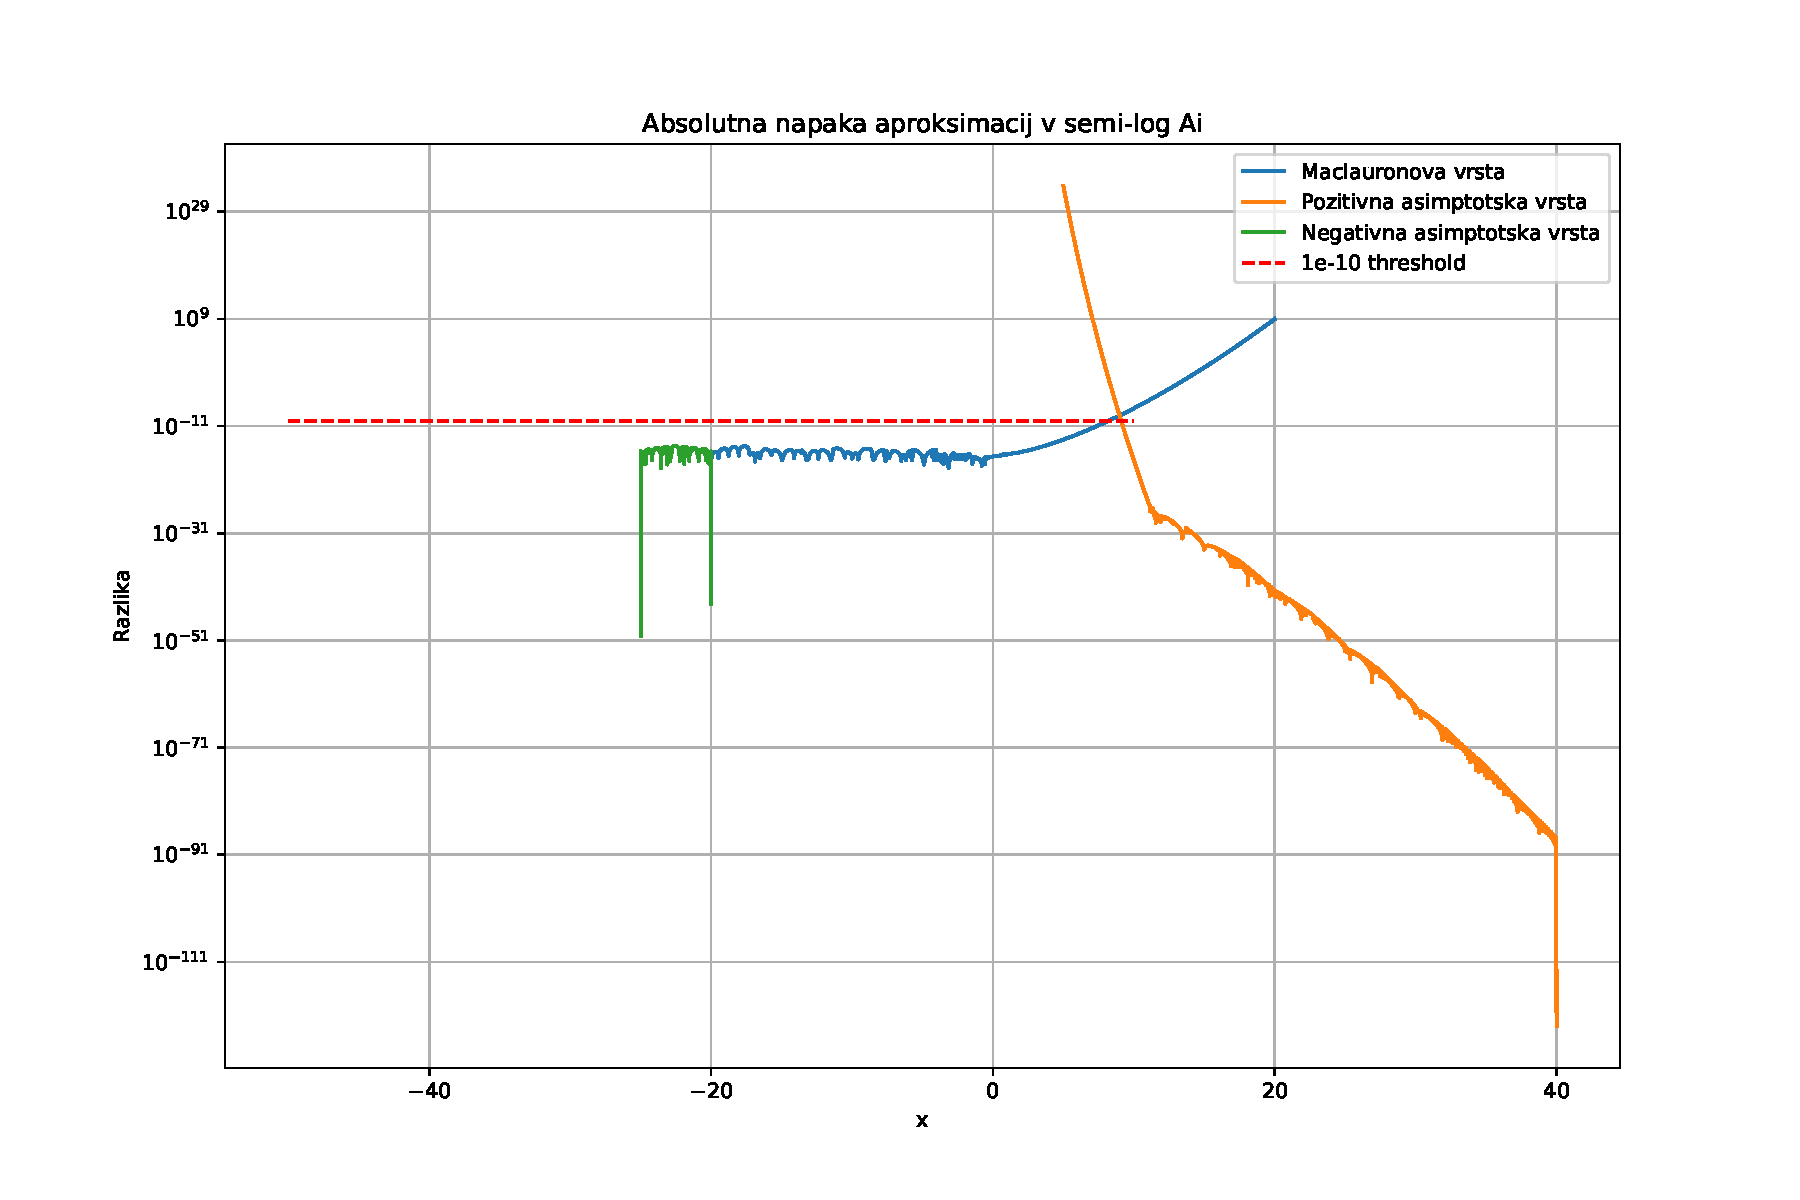
\includegraphics[width=0.7\textwidth]{ai_abs.pdf}
	\end{center}
\end{figure}

\begin{figure}[ht]
	\begin{center}
		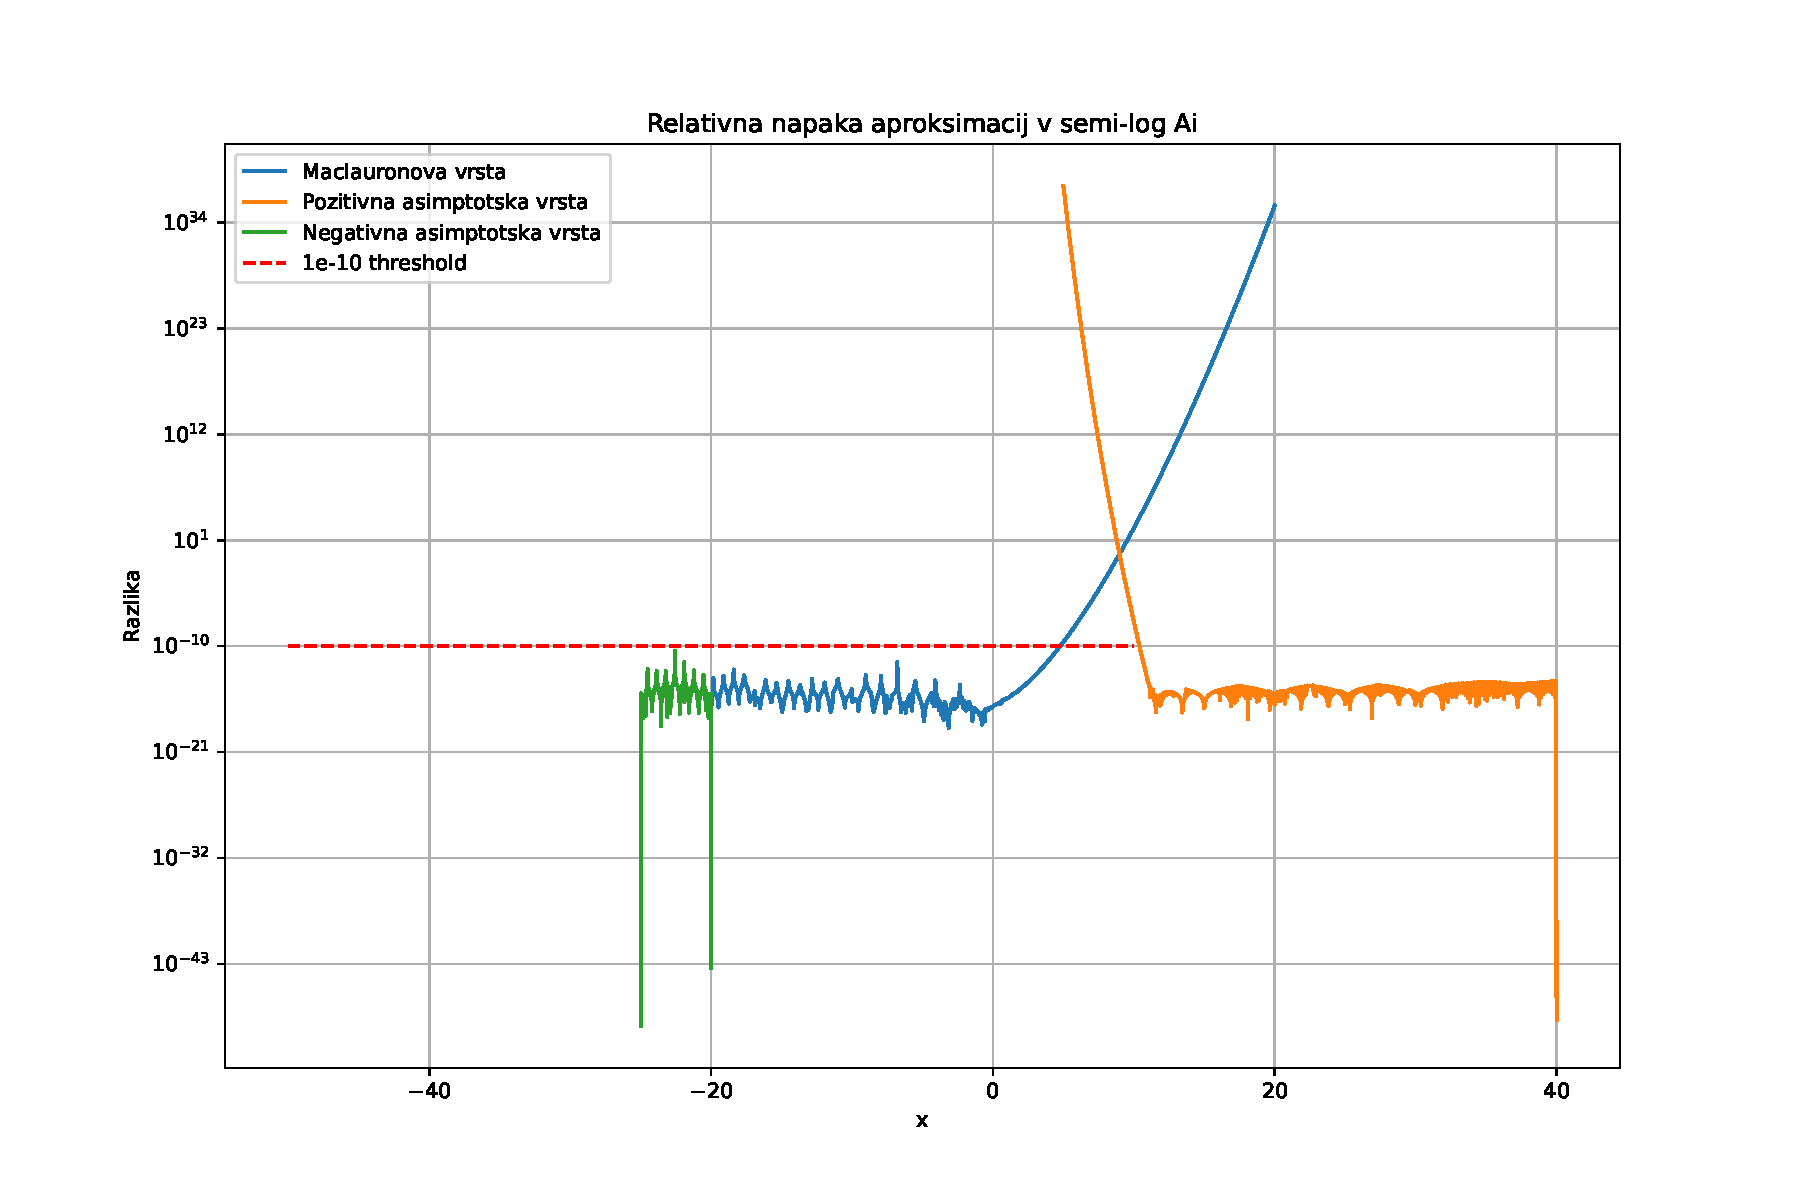
\includegraphics[width=0.7\textwidth]{ai_rel.pdf}
	\end{center}
\end{figure}

\newpage

\subsection{Funkcija Bi}
Iz grafa za absolutno napako je razvidno, da njegova vrednost divergira, kar je ravno nasprotno od funkcije $\Ai$.
Nasprotno vedenje lahko pričakujemo, saj se sami funkciji obnašata čisto drugače v pozitivnih eksremih, 
ena se ustali in konvergira proti $0$, med tem ko druga ekplodira v $\infty$. Ampak ko pogledamo relativno napako,
vidimo da se ne spreminja in je konstantno pod vrednostjo $10^{-10}$, kar je praktično identično vedenje, kot pri 
funkcij $\Ai$.

\begin{figure}[ht]
	\begin{center}
		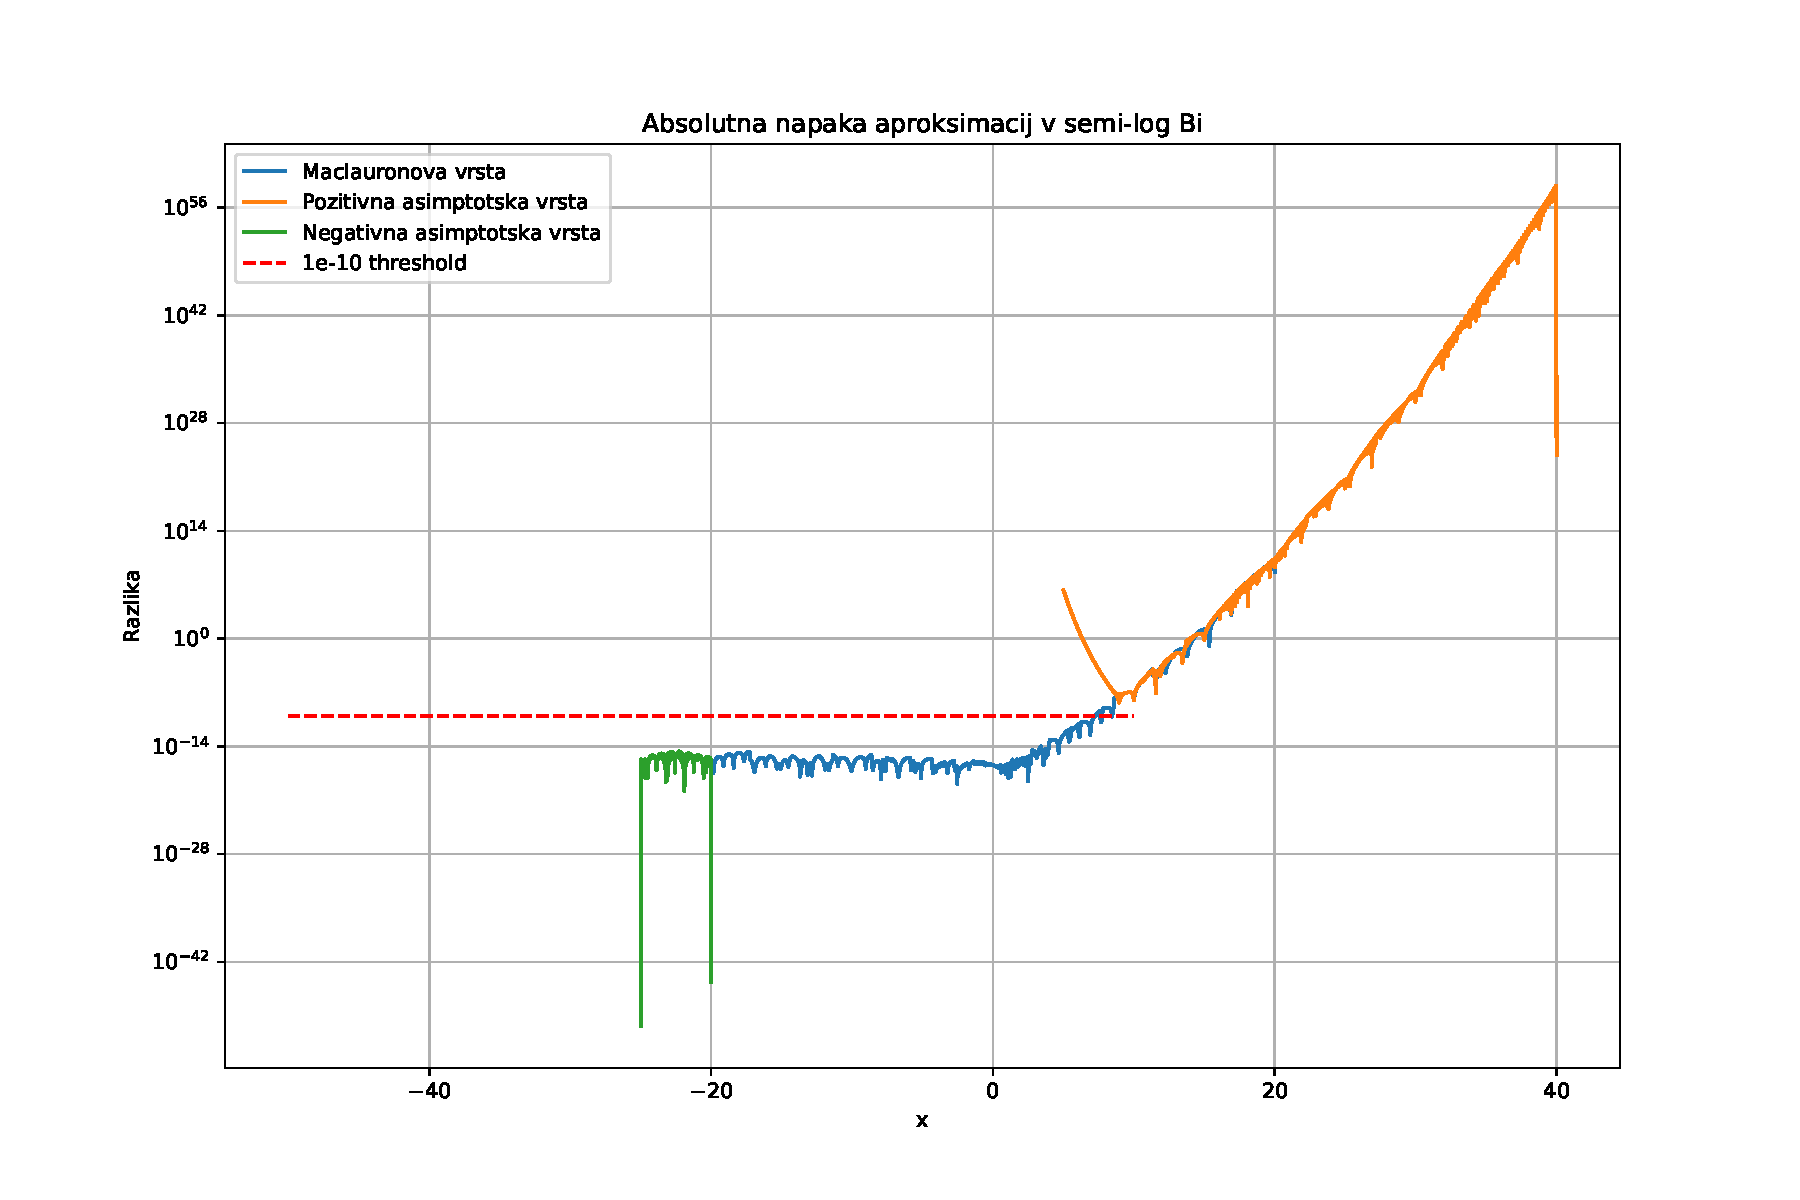
\includegraphics[width=0.7\textwidth]{bi_abs.pdf}
	\end{center}
\end{figure}

\begin{figure}[ht]
	\begin{center}
		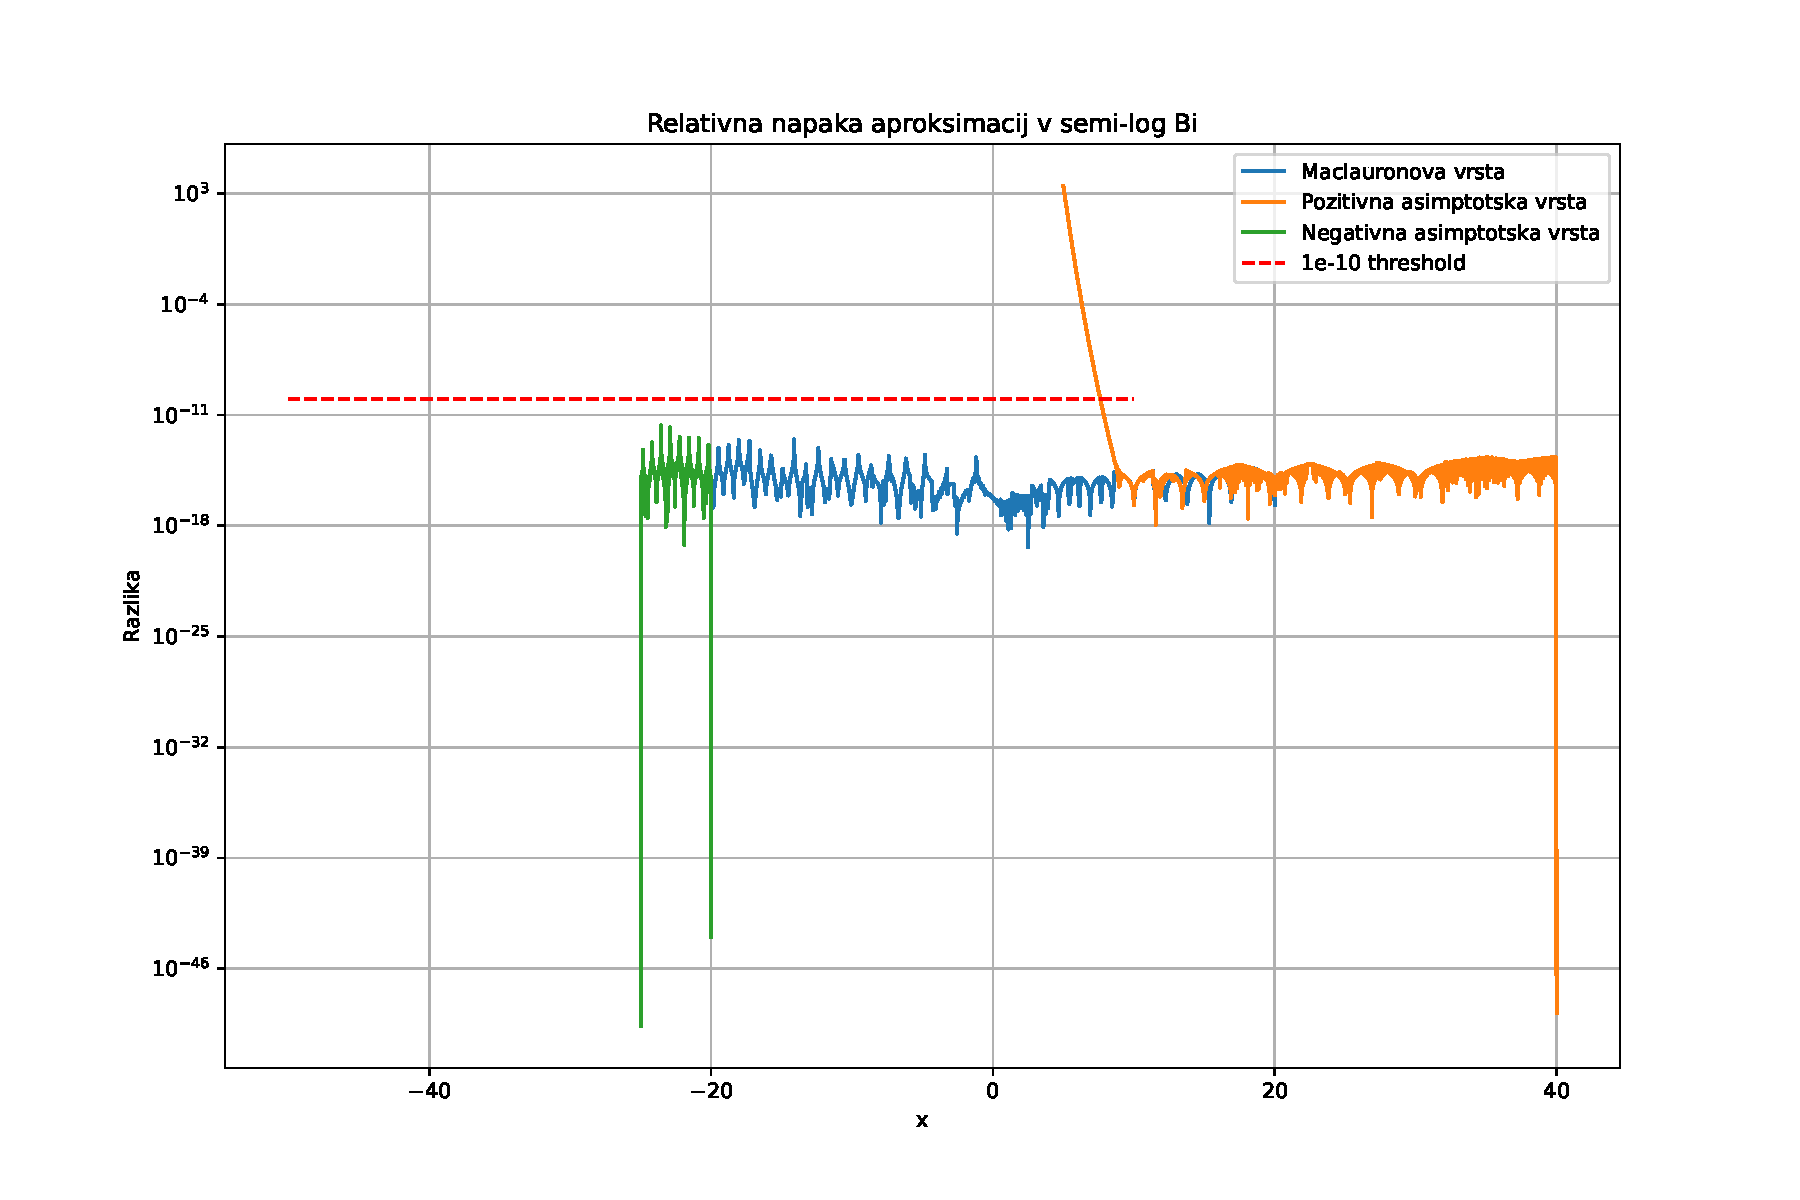
\includegraphics[width=0.7\textwidth]{bi_rel.pdf}
	\end{center}
\end{figure}

\newpage
\section{Izpolšave}
Mogoče najbolj trivialna izpolšava, bi bila znižanje 
natančnost mest, saj bi s tem pohitril računanje. Poleg tega, bi lahko pogledal
kakšno odstopanje ima sami referenčni funkciji glede na ta pravi $\Ai, \Bi$. Lahko bi tudi dodal logiko, ki bi 
mi omejila, do katerega člena bi računal svojo vrsto, s tem bi si prihranil čas, ki bi ga drugač uporabil za
prazno računanje. Naletel sem tudi na težavo, da so zelo velike številke v pythonu interperirane kot neskončno.
Ta problem bi se dalo rešiti, če bi računal svoje vrednosti pod logaritmom.

\section{Zakluček}
Opazil sem, da pri relativnem odsopanju je preprosto priti do vrednosti pod $10^{-10}$, pri funkciji $\Ai$ in $\Bi$.
Absolutna napaka, se pa obnaša dosti drugače, pri $\Ai$ se spušča in pri $\Bi$ raste čez vse meje.


\end{document}
